\usepackage{pdfpages}
\begin{document}
\date{April 2023}
\title{Greedy Subspace Localization}
\subtitle{(TODO: Better Title)}
\author{Akhil Sadam$^1$, Dr.Tan Bui Thanh$^2$}
\address{$^1$Department of Aerospace Engineering and Engineering Mechanics, UT Austin\\$^2$The Oden Institute for Computational Sciences, UT Austin}
\ead{akhil.sadam@utexas.edu, tanbui@oden.utexas.edu}
\begin{indented}
\item[]April 2023
\end{indented}
\section{Motivation}
\subsection{Background}
Contrastive learning procedures commonly use out-of-distribution (OOD) samples to train classifiers, as in Dr. Hinton's recent work \cite{FFA23}.
OOD samples are also used to train regressive models. An example would be Monte-Carlo null-space estimation for large linear systems (cite, better example?).

No regressive OOD, or \italic{negative data} approaches are done in a greedy manner, and they do not separate regression from localization (is this true ?).
We define localization as the process of subspace generation and feature selection, and regression as the process of fitting a model to the selected features.

The following goals are met by our approach:
\begin{itemize}
\item Greedy Layerwise Learning 
\item Separation of Localization and Regression
\item OOD-based Data Augmentation for Localization
\end{itemize}

(not sure if I should go through the FFA and motivate this work, or go directly to the architecture.)
\subsection{FFA-styled Contrastive Learning}
Recall Dr. Hinton's recent work \cite{FFA23}:
|-
Assume a supervised problem with $m$ labels and $t$ test samples as below.
\[
\mathbf{X_{test}} = \{x_i \mid i \in 1,...,t \},\ \mathbf{Y_{labels}} = \{y_j \mid j \in 1,...,m \}
\]
PYTHON ffasup
In prediction mode, each test sample $x_i$ is combined with every label $y_j, \forall j\in 1,...,m$. The net [Fig.~\ref{fig:ffasup}] outputs $m$ predictions of $\hat{p}(y_j \mid x_i)$.
For a single-label classifier, the label with the highest probability is chosen.
To classify all samples the FFA requires $m*t$ runs.
Normalization is required after each layer to ensure that prior layer $\|a_{l-1}\|^2$ does not affect later layers.
Training is a greedy layer-by-layer approach.
-|
Clearly, regression is not possible with this architecture. Several adjustments will now be made to allow for regression.
Since $y_j$ cannot be input unless each layer is to calculate an integral, we remove the direct product, and learn $y_j$ directly, removing the final sigmoid activation.
Note the overall function of the Affine + Norm layer is to shape / localize the input space, and layer norms no longer work as a layerwise loss. 
We replace this with a localization layer, which is a standard Affine layer with a Lipschitz loss function.
Finally, we add regression layers, to replace the expectation, resulting in a contrastive layerwise-regression architecture, that can incorporate OOD sampling.
\section{Base Forward Decomposition (FD) for supervised regression}
\subsection{Architecture}
Assume a supervised problem where the y-function is to be learnt.
\[
\mathbf{D} = \{(x_i,y_i) \mid y_i = \mathbf{F_y}(x_i)\:\forall\:i \in 1,...,n \}
\]
A general 3-layer implementation is shown in Figure \ref{fig:fda}.
PYTHON fda
\subsection{Loss Functions and Training}
\subsubsection{Base Localizer Loss}
Given input, output vector spaces $X$ and $Y$, with an intermediate, localized space $Z$, we define the localizer and regressor as $L$, $R$:
Note $F_y$ denotes the mapping to be learnt (as before).
\[
L : X \rightarrow Z, R: Z \rightarrow Y, F_y : X \rightarrow Z.
\]
For noise-augmented x with a variance of $\delta$, 
\[
\epsilon_p \sim N(0,\delta^2)    
\]
\[
\hat{y_{aug}} = R(z), z = L(x + \epsilon_p)
\]
To localize the input space $X$ into $Z$, given an approximate Lipschitz constant, and a particular neighborhood size (a delta-ball), the following loss is used.
Note $\sigma$ denotes the ReLU function, and $\text{MSE}$ denotes mean-squared-error.
Both the prediction and the true y-value are lifted to a higher space by concatenation (denoted by $\oplus$) with the latent-space value $z$, so that the continuity condition imposed can work with discontinous functions.
\[
\mathbf{\text{Loss}_\text{localizer}(x,y)} = \sigma(\text{MSE}(\hat{y_{aug}} \oplus z,y \oplus z) - k^2 \delta^2)
\]
Note this condition follows directly from the Lipschitz continuity - that the output from the $\delta$-ball falls within the $k\delta$-ball.
The output ball is centered at the true y-value instead of the mean, due to computational ease; this also serves as a MSE addition.

\subsubsection{OOD Data Augmentation}
(TODO remove colloquial language)
To allow for contrastive learning, and accurately learn the `nullspace', or space not data-driven, negative-data is generated as follows:
\[
x_n = x + \epsilon_n
\]
\[
\|\epsilon_n\| = \delta + \epsilon_{\text{machine-precision}}, \text{in random direction}
\]

This negative data allows an additional localizer loss component:
\[
\mathbf{\text{Loss}_\text{localizer-negative}(x_n,y)} = \sigma( - \text{MSE}(\hat{y_{aug}} \oplus z,y \oplus z) + k^2 \delta^2)
\]

\subsubsection{Variance Expansion Loss (TODO)}
Greatly limited function behavior has been accounted for. For example, a maximum-variance expansion like PCA would be useful in some cases.
If neighbors in $Y$-space are considered, their set diameter in $Z$-space denoted $D$, the following results for some fixed $y \in Y$:
\[
\mathbf{D} = \text{diam} (L(f^{-1}_y(N_\varepsilon(y))))
\]
\float{
\includegraphics[width=1.0\linewidth]{./FDA/memo/plots/functionbehavior.jpg}
\label{fig:functionbehavior}
}
(TODO need another picture for X,Y,Z relationship with delta,epsilon-balls)
(TODO replace photo, change A to Z)
(TODO add loss for variance-expansion)
(TODO rewrite with more text)

\subsubsection{Regressor Loss}
On the regression side, a straightforward MSE loss is implemented.
\[
\mathbf{\text{Loss}_\text{regressor}(x,y)} = \text{MSE}(\hat{y_{aug}},y)
\]

\subsubsection{Layerwise Training}
Notice the above deals with a single layer. Several layers can be stacked and trained in a greedy fashion, by freezing prior weights and learning the residual.

\subsubsection{Complete Algorithm}
(TODO rewrite above in a algorithm form)

\subsection{Theorems?}
Note this method is similar to ResNet, so can we avoid gradient issues?
Any convergence theorems?
\subsection{UQ?}
Uncertainty quantification?

\subsection{Results}
We use standard ReLU layers for the localizer and linear layers for the regressor. \ref{fig:fda} gives the following.
PYTHON fda2

(TODO - rewrite section with curated examples once the algorithm is finalized)

\subsubsection{Convergence Rates at different frequencies with noisy data}

\includepdf[pages=-]{./FDA/memo/plots/data_041623/hf_lf_v2.pdf}


\subsubsection{Comparison with DNN}

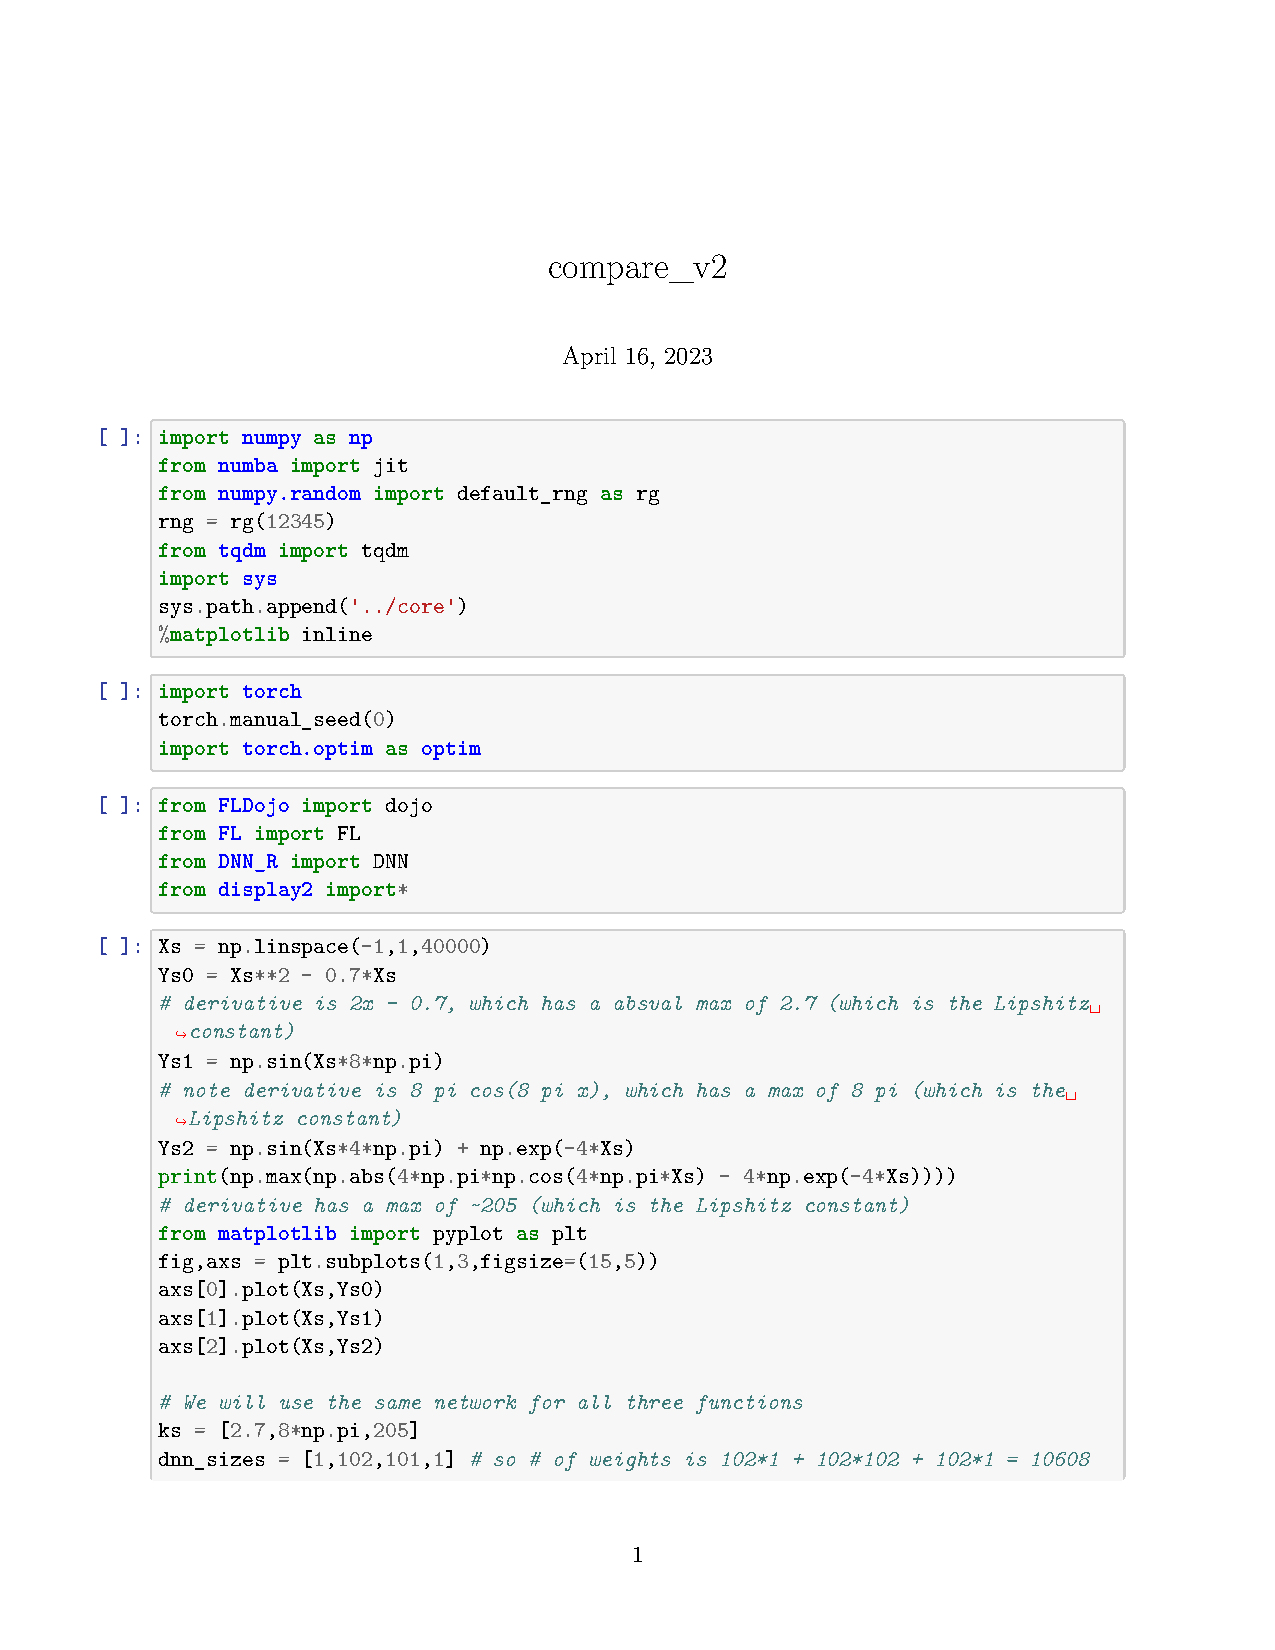
\includepdf[pages=-]{./FDA/memo/plots/data_041623/compare_v2.pdf}

\section{Forward Decomposed PDE-Inverter (Data-Free)}

TODO : from this point on, everything is just notes (rewrite)! 

\float{
\includegraphics[width=1.0\linewidth]{./FDA/memo/plots/srd01.jpg}
\label{fig:srd01}
} 

\newpage

\float{
\includegraphics[width=1.0\linewidth]{./FDA/memo/plots/datafree.jpg}
\label{fig:datafree}
}
- Use FD to learn a T-Net (autoencoder), with a generative FD variant for the forward pass.
- Goal is low-data semi/un-supervised learning, with OOD-based data augmentation.
- Test on wafer scratch/defect detection?
- Use a good noise model in forward pass to quantify uncertainty. (do a probability analysis)
- Use ELBO loss and possibly wavelet encoding from Paris Perdakis' work to make it resolution-independent.
- Use fractal theory to learn fracture patterns in materials.

\section{Forward Decomposed PDE-GAE (generative autoencoder)}
- Now move to semi-sup PDE learning

\section{PDE-UQ}
\subfloat{
\includegraphics[width=1.0\linewidth]{./FDA/memo/plots/uq.jpg}
\label{fig:uq}
}

\section{Appendix}
% \sfig{FFA/memo/plots/DNN}{DNN Baseline}
\subsection{PAST DATA WITH ERRORS!}
\subsubsection{data 041523}
Known ERRORS:
\begin{itemize}
    \item Localizer loss had $k\delta$ instead of $k^2 \delta^2$. 
\end{itemize}
files affected:

\begin{itemize}
\item compare.ipynb
\item fl greedy, fl sine, fl stability.ipynb
\item fl, fl2, fl3, fl4, fl5.ipynb
\end{itemize}

PDF:./FDA/memo/plots/data_041523/compare.pdf

% 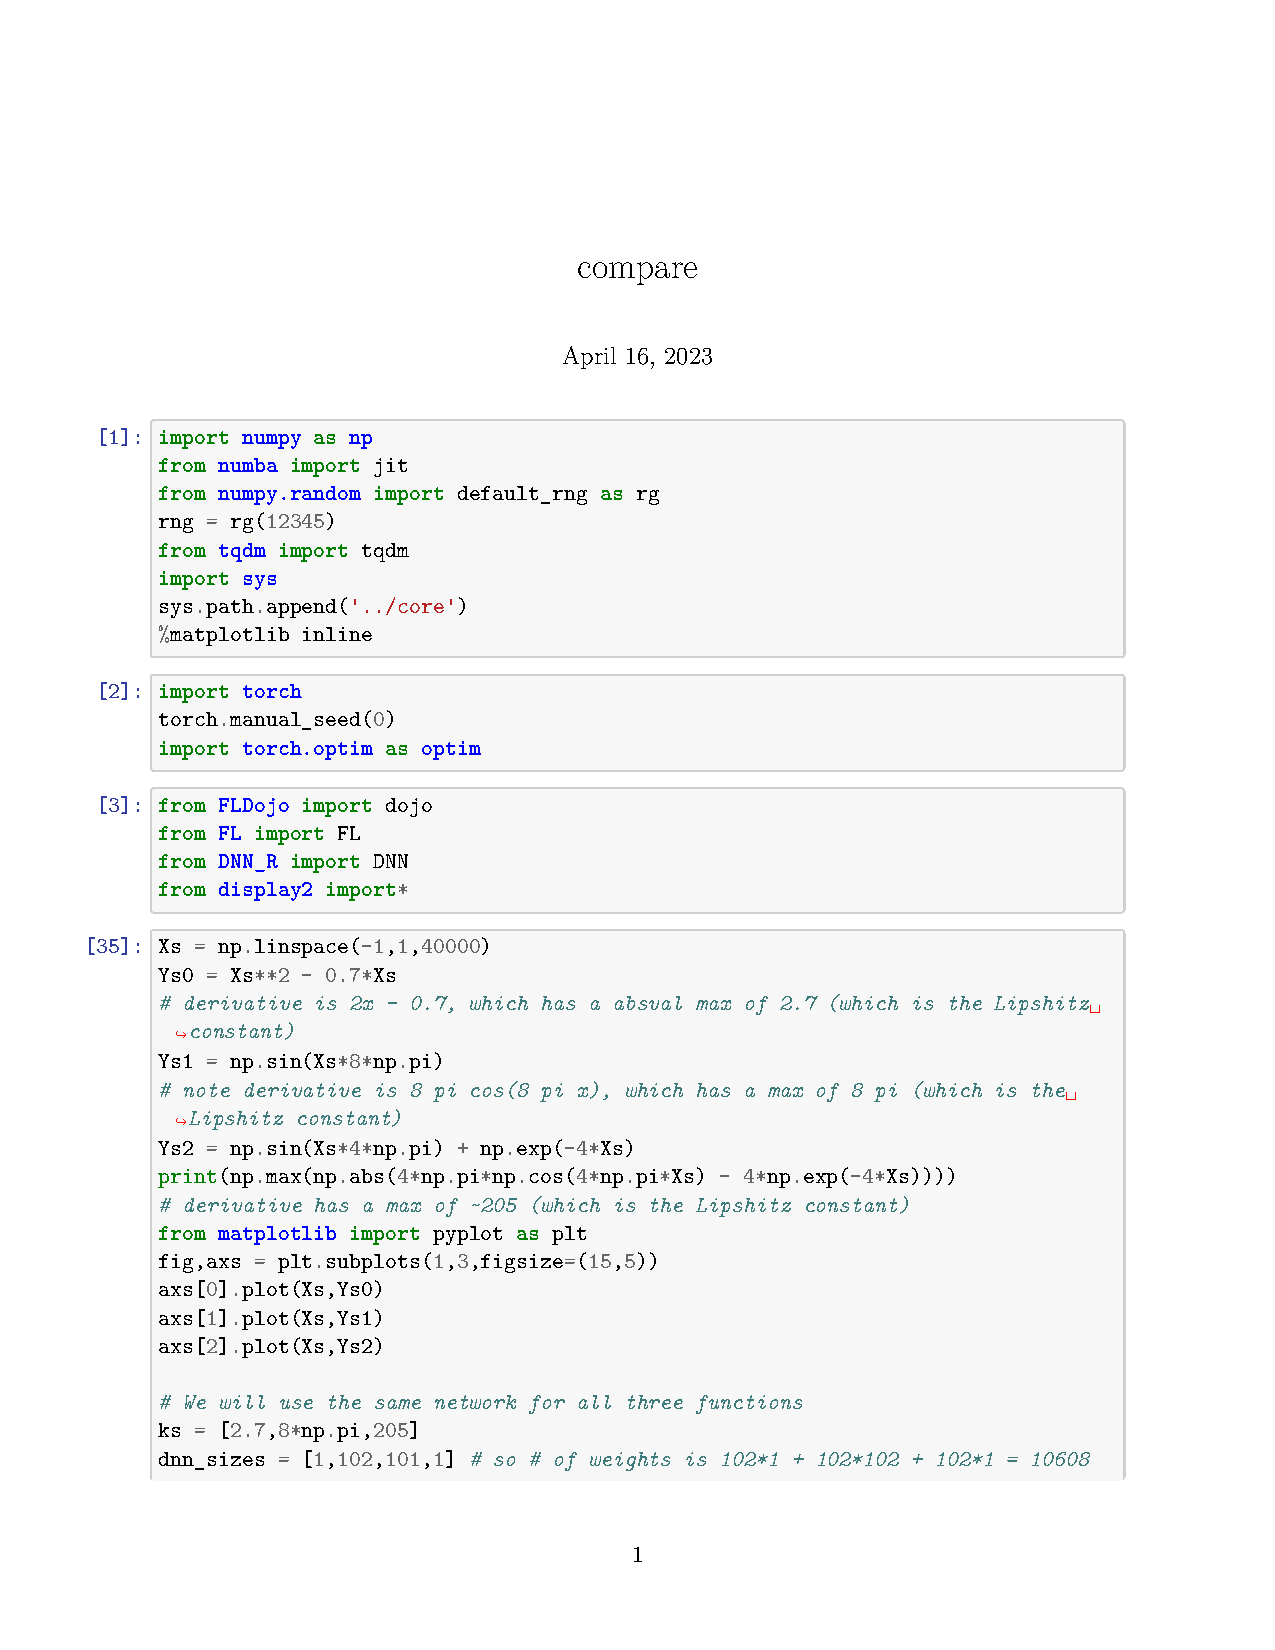
\includepdf[pages=-]{./FDA/memo/plots/data_041523/compare.pdf}

\section{Acknowledgements}
Inspired by Dr. Hinton's paper \cite{FFA23}.
This work follows from a discussion with Mr. C G Krishnanunni and Mr. Wesley Lao.
\section{References}
\bibliography{References}
\end{document}